\subsection{Phase-Aligned STDB Construction (RQ1)}
\label{sec:methods-data}

We collect match records from the official PUBG Developer API
\cite{pubgDeveloperPortal,pubgTelemetryGuide}. The telemetry file is an event
stream with time, actor, location, and game-state context
\cite{pubgTelemetryEvents,pubgTelemetryObjects}. The study population contains
21,824 matches and spans twelve maps and all standard team modes---solo, duo,
and squad, in first- and third-person perspectives---with third-person squad
matches forming the largest share (15,213). Table~\ref{tab:api-fields}
summarizes how we use the raw records.

\begin{table*}[t]
\centering
\caption{Raw telemetry meaning and analysis representation.}
\label{tab:api-fields}
\small
\begin{tabular}{p{0.27\linewidth}p{0.31\linewidth}p{0.34\linewidth}}
\toprule
Raw information & Meaning in the match & Representation \\
\midrule
Match and roster context & Map, mode, duration, team membership, outcome. &
Match/team records; auxiliary placement target. \\
Timestamped player state & Location, health, alive status, vehicle state. &
Moving players, team centroids, state and movement features. \\
Zone state over time & Safe-zone and blue-zone centers, radii, timing. &
Dynamic regions, phase intervals, exposure features. \\
Combat and elimination events & Attacker-victim interaction with time, place,
and damage context. & Spatial events, elimination times, combat relations. \\
Resource and support events & Equipment, resource use, healing, boosting. &
Readiness summaries by team and phase. \\
Common time and location metadata & Coordinates linking separate records. &
Shared axes for trajectories, regions, events, and edges. \\
\bottomrule
\end{tabular}
\end{table*}

The API gives events, not analysis objects. We therefore convert the stream
into four object types on two shared axes: elapsed match time and a common map
plane. Player positions, resampled on a 10-second grid, become team centroids,
that is, moving objects. Safe- and blue-zone states become phase-indexed
dynamic regions. Combat and elimination records become spatial events anchored
to a time and a place. Phase boundaries become explicit intervals
\([a_k,b_k]\), with the pre-zone landing interval indexed as phase 0.
Concretely, the STDB is the set of relations in
Table~\ref{tab:stdb-schema}; team-phase features, labels, and edges are
interval aggregations---joins of team states, spatial events, and zone
geometry restricted to \([a_k,b_k]\).

\begin{table}[t]
\centering
\caption{Conceptual STDB schema. \(m\): match, \(i,j\): teams, \(k\): phase,
\(t\): time, \(r\): relation type.}
\label{tab:stdb-schema}
\small
\begin{tabular}{llp{0.45\linewidth}}
\toprule
Relation & Key & Contents \\
\midrule
Match & \(m\) & map, mode, duration \\
Team & \(m,i\) & roster size, outcome \\
Phase & \(m,k\) & interval \([a_k,b_k]\); safe/blue-zone geometry \\
Team state & \(m,i,t\) & centroid, alive count, health, vehicle \\
Spatial event & \(m,e\) & time, place, attacker/victim teams, kind, damage \\
Team-phase & \(m,i,k\) & 66 features; hazard label \\
Edge & \(m,k,r,i,j\) & weight of relation \(r\) \\
\bottomrule
\end{tabular}
\end{table}

Table~\ref{tab:data-funnel} reports the conversion funnel. Almost the entire
gap between retrieved and graph-ready matches consists of tutorial and
training-range sessions (5,658 matches), which are not competitive play and
are excluded by design. Only nine further matches drop out, due to degenerate
telemetry such as missing position traces or too few phases to define a
next-phase label.

\begin{table}[t]
\centering
\caption{Data funnel from raw telemetry to graph-ready matches.}
\label{tab:data-funnel}
\small
\begin{tabular}{lr}
\toprule
Stage & Matches \\
\midrule
Official telemetry retrieved & 27,491 \\
Converted to STDB & 21,833 \\
Team positions available & 21,830 \\
Team-phase features available & 21,830 \\
Next-phase labels available & 21,824 \\
Team-relation edges available & 21,830 \\
Graph-ready matches, \(N_{\max}=128\) & 21,824 \\
\bottomrule
\end{tabular}
\end{table}

\subsection{Team-Phase Features (RQ1)}
\label{sec:methods-features}

The modeling unit is the team-phase tuple \((m,i,k)\): match \(m\), team
\(i\), phase \(k\). Each row summarizes one team's trajectory, zone exposure,
combat, and readiness during one phase; every quantity in a row is computed
from observations within that phase, and nothing crosses its end boundary.
Team positions are centroids over members not yet eliminated,
\(c_{i,t}=|P_{i,t}|^{-1}\sum_{p\in P_{i,t}}\ell_{p,t}\), where \(\ell_{p,t}\)
is player \(p\)'s location; centroids simplify a split squad, so team spread
and minimum enemy distance appear as features in the same row to compensate.
All zone-relative quantities (movement alignment, zone entry time, time
outside the zone) refer to the target safe zone announced during phase \(k\)
itself, which is visible to players throughout the phase; no future zone is
used. Figure~\ref{fig:team-phase-feature-example} shows the view that one row
captures. Under the habitat-contraction lens of
Section~\ref{sec:related-work}, safe-zone exposure and nearby-team pressure
are not background details; they are part of the team's risk state.

\begin{figure}[t]
\centering
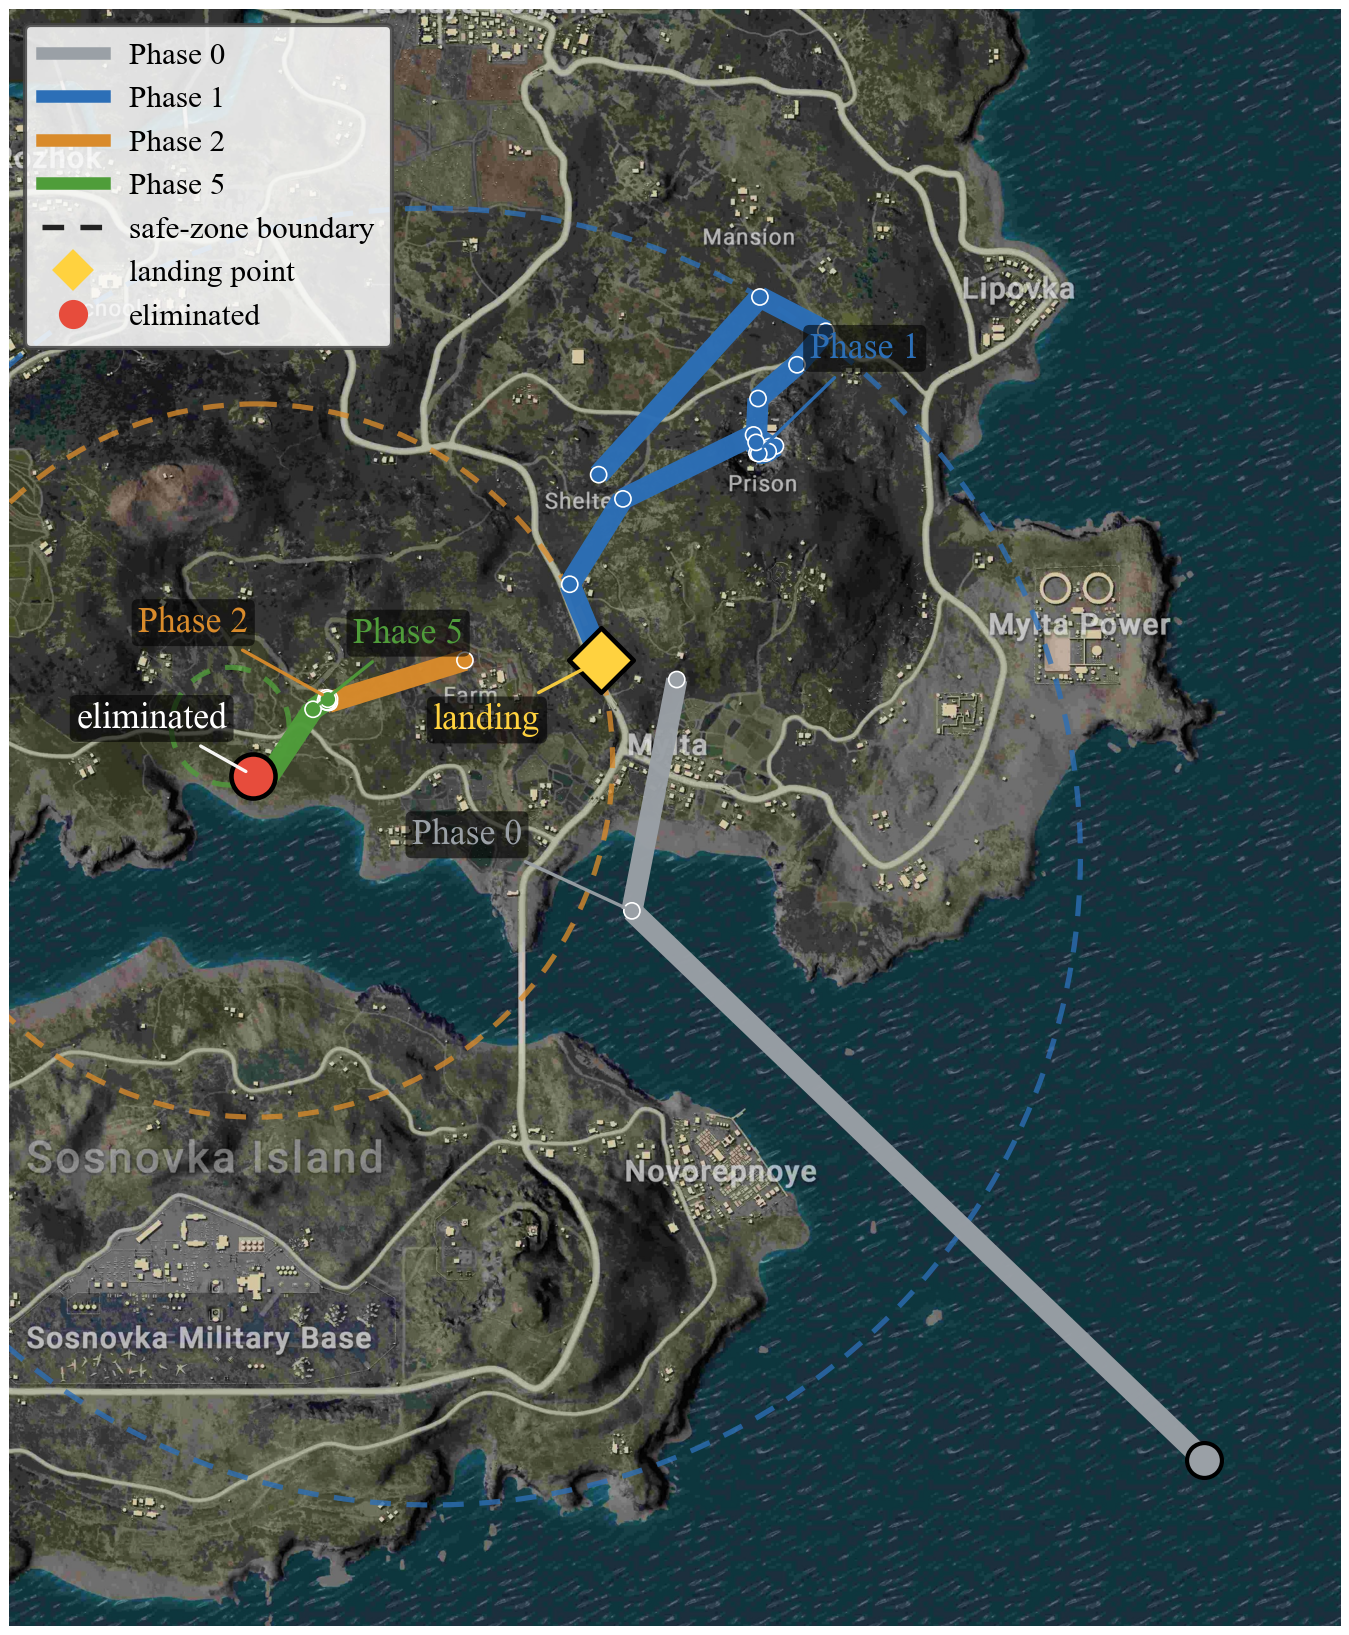
\includegraphics[width=0.48\textwidth]{figures/team_phase_feature_example.png}
\caption{PUBG gameplay as a spatio-temporal process. Solid line segments show
one team's centroid movement during selected phases, and dashed circles of the
same color show the corresponding target safe-zone boundaries on the Erangel
battlefield. Phase 0 denotes the pre-zone landing interval, the yellow diamond
marks the landing point, and the red marker denotes elimination.}
\label{fig:team-phase-feature-example}
\end{figure}

Table~\ref{tab:feature-groups} separates conventional telemetry aggregates
from the added STDB spatio-temporal features. The complete dictionary of all
66 node features, with the definition and scaling of each, is given in
Appendix~\ref{app:features}. The \(d\) column reports the raw tabular variable
count used in the HGB representation ablation; DynamicSTGNN uses normalized
numeric variants of the same sources as a 66-dimensional node feature vector.
The STDB-only count includes the shared phase index, which is counted once in
the combined view. Each quantity is scaled by a fixed, feature-specific
constant. Variables that can occasionally take very large values, such as
damage, item pickups, and combat-event counts, are log-compressed; the scales
are constants of the representation, not statistics fitted on training data.

\begin{table}[t]
\centering
\caption{Conventional telemetry aggregates and added STDB spatio-temporal
features.}
\label{tab:feature-groups}
\scriptsize
\setlength{\tabcolsep}{2.5pt}
\begin{tabular}{p{0.18\linewidth}p{0.22\linewidth}rp{0.42\linewidth}}
\toprule
Source & Group & \(d\) & Representative quantities \\
\midrule
Conventional & Phase/team state, combat, readiness & 57 &
Phase index and duration, alive teams/players, zone radii and center shift,
health, team spread, vehicles, damage, knockdowns, kills, items, healing/boost
use. \\
Added STDB & Trajectory, zone/enemy exposure & 16 &
Team-centroid path length, displacement, sinuosity, speed, rotation timing,
safe-zone alignment and entry time, boundary distance, outside-zone ratio,
enemy density, nearest-enemy distance, combat-area passage. \\
Combined view & Conventional+STDB & 72 &
Tabular hazard-prediction view combining conventional aggregates with STDB
trajectory/exposure features. \\
\bottomrule
\end{tabular}
\end{table}

\subsection{Dynamic Team Graphs (RQ1)}
\label{sec:team-graphs}

The third representation object makes inter-team relations explicit. For
phase \(k\) we define a weighted heterogeneous graph
\(G_k=(V_k,X_k,\{A_k^r\}_{r\in R})\), where \(V_k\) is the set of co-observed
teams, \(X_k\) is the team-phase feature matrix of
Subsection~\ref{sec:methods-features}, and \(A_k^r\) is the weighted
adjacency matrix of relation \(r\)~\cite{sanchezLengeling2021gnnIntro}. A
match is therefore a discrete-time dynamic graph: a sequence
\(G_1,\dots,G_T\) of snapshots, one per phase, in which nodes drop out as
teams are eliminated. All edges are computed from phase-\(k\) observations
only.

The relation set \(R\) has three channels:
\[
A^{\mathrm{prox}}_{ij,k}=e^{-\bar d_{ij,k}/\lambda},\qquad
A^{\mathrm{comb}}_{ij,k}=\log\!\big(1+D_{ij,k}+\gamma_e E_{ij,k}+\gamma_k K_{ij,k}\big),
\]
\[
A^{\mathrm{press}}_{ij,k}=\rho_{ij,k}\, e^{-\bar d^{\,\mathrm{p}}_{ij,k}/\lambda},
\]
where \(\bar d_{ij,k}\) is the mean centroid distance between teams \(i\) and
\(j\) during the phase; \(D\), \(E\), and \(K\) are the damage, eliminations,
and knockdowns dealt by \(i\) to \(j\); a team is under zone pressure when it
is outside the safe zone or within \(\tau_b\) of its boundary;
\(\rho_{ij,k}\) is the fraction of the phase that both teams jointly spend
under pressure within \(\tau_d\) of each other; and \(\bar d^{\,\mathrm p}\)
averages distance over those moments. Proximity is symmetric and complete (no
hard distance cutoff), co-pressure is symmetric and sparse, and combat is
directed and sparse. The constants are fixed a priori at map scale,
\(\lambda=200\)\,m, \(\gamma_e=100\), \(\gamma_k=50\), \(\tau_b=150\)\,m,
\(\tau_d=200\)\,m; we did not tune them, and sensitivity to these choices is
discussed in the limitations. Averaged over phases 1--8, a phase graph
contains about 14 co-observed teams, with about 14 directed combat edges and
7 co-pressure pairs per phase.

Each channel is row-normalized,
\(\bar A^{r}_{ij,k}=A^{r}_{ij,k}/\sum_{j'}A^{r}_{ij',k}\), with edgeless rows
staying zero; the proximity channel carries self-loops, and padded or
eliminated teams carry no edges at all. Two conventions matter for reading
the model. First, combat is stored with the attacker as the row: in the
aggregation \(\bar A H\), an attacking team aggregates the state of the teams
it damaged, while the converse signal---being attacked---is carried by the
combat-taken node features. Second, row normalization removes scale
differences in aggregation; absolute combat intensity is retained in
node-level combat features, so the combat adjacency encodes the distribution
of engagement partners rather than raw magnitude.
Figure~\ref{fig:dynamic-graph-example} illustrates the conversion.

\begin{figure*}[t]
\centering
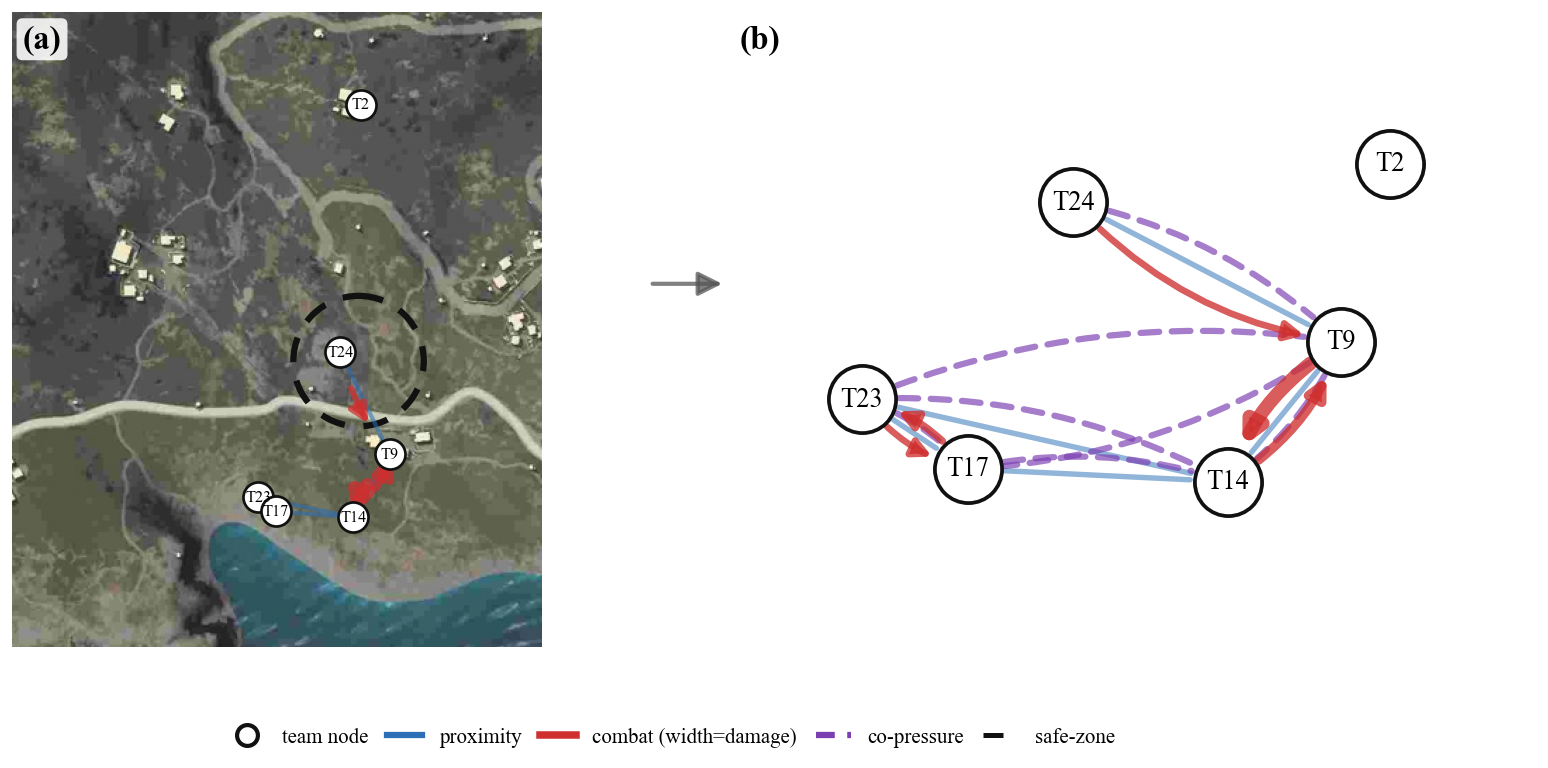
\includegraphics[width=0.86\textwidth]{figures/dynamic_heterogeneous_graph_example.png}
\caption{Visual conversion of a phase-level STDB snapshot into a dynamic team
graph for one PUBG phase. Panel (a) shows team centroids on the Erangel map,
the current safe-zone boundary, and combat events. Panel (b) keeps the same
teams and relations but removes the map background, leaving only the graph
structure used by the model.}
\label{fig:dynamic-graph-example}
\end{figure*}

This design has four properties we rely on. Heterogeneous channels keep
distinct risk mechanisms separate---being near a team, being shot by it, and
being pushed into the same shrinking space are different relations---and let
the model weigh them rather than conflating them in a single graph. The
complete weighted proximity channel avoids a distance-threshold
hyperparameter and preserves the full ordering of distances; it risks
over-smoothing in team-dense early phases, but the exponential decay
concentrates mass on nearby teams, and the no-edge and shuffle controls of
Subsection~\ref{sec:dynamic-team-graph-model} bound how much of any gain
could come from indiscriminate mixing. Directed combat edges retain who
initiated an interaction. Finally, snapshot dynamics align the graph clock
with the phase clock of the hazard task, and row normalization keeps neighbor
aggregation comparable as the number of surviving teams shrinks across
phases.
